\documentclass[a4paper,11pt,twoside]{article}
%\documentclass[a4paper,11pt,twoside,se]{article}

\usepackage{UmUStudentReport}
\usepackage{verbatim}   % Multi-line comments using \begin{comment}
\usepackage{courier}    % Nicer fonts are used. (not necessary)
\usepackage{pslatex}    % Also nicer fonts. (not necessary)
\usepackage[pdftex]{graphicx}   % allows including pdf figures
\usepackage{listings}
\usepackage{pgf-umlcd}
\usepackage{blindtext}
\usepackage{enumitem}
%\usepackage{lmodern}   % Optional fonts. (not necessary)
%\usepackage{tabularx}
%\usepackage{microtype} % Provides some typographic improvements over default settings
%\usepackage{placeins}  % For aligning images with \FloatBarrier
%\usepackage{booktabs}  % For nice-looking tables
%\usepackage{titlesec}  % More granular control of sections.

% DOCUMENT INFO
% =============
\department{Department of Computing Science}
\coursename{Parallel Programming 7.5 p}
\coursecode{5DV152}
\title{Exercises, Chapter/Topic 1}
\author{Lorenz Gerber ({\tt{dv15lgr@cs.umu.se}} {\tt{lozger03@student.umu.se}})}
\date{2017-01-26}
%\revisiondate{2016-01-18}
\instructor{Lars Karlsson / Mikael Ränner}


% DOCUMENT SETTINGS
% =================
\bibliographystyle{plain}
%\bibliographystyle{ieee}
\pagestyle{fancy}
\raggedbottom
\setcounter{secnumdepth}{2}
\setcounter{tocdepth}{2}
%\graphicspath{{images/}}   %Path for images

\usepackage{float}
\floatstyle{ruled}
\newfloat{listing}{thp}{lop}
\floatname{listing}{Listing}



% DEFINES
% =======
%\newcommand{\mycommand}{<latex code>}

% DOCUMENT
% ========
\begin{document}
\lstset{language=C}
\maketitle
\thispagestyle{empty}
\newpage
\tableofcontents
\thispagestyle{empty}
\newpage

\clearpage
\pagenumbering{arabic}

\section{Introduction}
This report is part of the mandatory coursework. It describes the solutions for several chosen exercises from the course book \cite{pacheco2011}.
\section{2.4 - Counting pages}
$2^{20}$
\section{2.8 - Hardware multithreading and caches}
Caching operates on whole cache lines. Hence if the chance that another process/thread changes something in a specific cache line increases with cache size and number of processes/threads. The specific situation that can happen is called `false sharing': When one process changes data in a cache line, there is no possibilty to check or know for another process which data exactly was changed. It can very well be the case that to the current process unrelated data was changed and a cache reload would not be needed. However, cache has to be reloaded. 
\section{2.10 - Communication overhead}
The calculations can be split in two parts: the instructions and the communication. For both a) and b) the instructions will take the same time:\\
\verb+instructions / cores / instructions_per_second+\\
Hence $10^{12} \div 1000 \div 10^{6} = 1000 sec$. For communications, the time is calculated as\\
\verb+messages_to_send * time_per_message+\\
while messages to send is described as $10^{9}(p-1)$. 
\begin{enumerate}[label={\alph*)}]
\item if sending one message takes $10^{-9}$ seconds, the communication with 1000 cores will take: $10^{9}(1000-1) \times 10^{-9} = 99'900 sec$, together with the actual calculation, $100'900 sec = 28.03h$.
\item if sending one message takes $^{-3}$ seconds , the communication with 1000 cores will take: $10^{9}(1000-1) \times 10^{-3} = 99'900'000'000 sec$, together with the actual calculation, $99'900'001'000 sec = 3'167.8 years$.
\end{enumerate}


    
\section{2.16 - Speedup efficiency}
To calculate the hypothetical speed up between a serial and parallel program with the run time formulas $T_{serial}=n^{2}$ and $T_{parallel} = \frac{n^{2}}{p}+log_{2}(p)$ where $T=[ms]$, a short program was written that calculates the speedup $S=\frac{T_{serial}}{P_{parallel}}$. The obtained data was then plotted (\textit{figure \ref{fig:speedup}}) using the R statistical environment \cite{rlanguage}.

\begin{verbatim}
#include <stdio.h>
#include <stdlib.h>
#include <math.h>

#define START_N 10
#define START_P 1
#define N_LENGTH 6
#define P_LENGTH 8

int main (void) {
  
  FILE *f = NULL;
  if((f = fopen("data.txt", "w"))<0){
    perror("fopen");
    exit(EXIT_FAILURE);
  }

  double n = START_N;
  double p = START_P;

  double speedUp = 0;

  for(int i = 0 ; i < N_LENGTH; i++){
    for(int j = 0; j < P_LENGTH; j++){

      speedUp = n*n / ((n * n) /  p  + (log(p)/log(2)));
      fprintf(f, "%lf\t", speedUp);
      printf("SpeedUp for n = %lf p = %lf is %lf\n", n, p, speedUp);
      p*=2;
    }

    fprintf(f, "\n");
    n*=2;
    p = START_P;
  }

  fclose(f);
  return 0;
}
\end{verbatim}

\begin{enumerate}[label={\alph*)}]
\item In table \ref{tab:speedup}, the rawdata is presented, while figure \ref{fig:speedup} shows graphs for constant \verb+n+ (upper graph) and constant \verb+p+ (lower graph) respectively. From the upper graph, it can be seen that for constant \verb+p+, the growth of speedup for larger and larger problem instances \verb+n+ decreases and eventually closes in to a horizontal asymptote. The lower graph shows, that for large problem sizes \verb+n+, increasing the number of cores \verb+p+ leads to almost linear speedups, while when we increase the number of cores for small problem instances, the speed up levels of very soon.    

\item Efficency is defined as $E = \frac{T_{serial}}{pT_{parallel}}$. In the current question, $T_{parallel}$ is defined as $\frac{T_{serial}}{p}+T_{overhead}$. Hence efficency $E$ translates here to $\frac{T_{serial}}{p(\frac{T_{serial}}{p}+T_{overhead})} = \frac{T_{serial}}{T_{serial}+pT_{overhead}}$. From the last expression, it can be seen, that if $p$ is held constant and $T_{serial}$ grows faster than $T_{overhead}$, the ratio will increase, hence the efficency increases.
The opposite follows, that if $T_{overhead}$ grows monotoically faster than $T_{serial}$, it will sooner or later dominate the denominator, the ratio will decrease, hence the efficency decrease.
  
\end{enumerate}
\begin{table}[ht!]
\centering
\caption{\textit{shows the speed ups in relation to p (vertical) and n (horizontal)}}
\label{tab:speedup}
\begin{tabular}{l|cccccccc}
p \textbackslash n & \multicolumn{1}{l}{1} & \multicolumn{1}{l}{2} & \multicolumn{1}{l}{3} & \multicolumn{1}{l}{4} & \multicolumn{1}{l}{5} & \multicolumn{1}{l}{6} & \multicolumn{1}{l}{7} & \multicolumn{1}{l}{8} \\ \hline
1                  & 1                     & 1.96                  & 3.70                  & 6.45                  & 9.76                  & 12.31                 & 13.22                 & 12.85                 \\
2                  & 1                     & 1.99                  & 3.92                  & 7.55                  & 13.79                 & 22.86                 & 32.65                 & 39.51                 \\
3                  & 1                     & 2                     & 3.98                  & 7.88                  & 15.38                 & 29.09                 & 51.61                 & 82.05                 \\
4                  & 1                     & 2                     & 4                     & 7.97                  & 15.84                 & 31.22                 & 60.38                 & 112.28                \\
5                  & 1                     & 2                     & 4                     & 7.99                  & 15.96                 & 31.80                 & 63.05                 & 123.67                \\
6                  & 1                     & 2                     & 4                     & 8                     & 15.99                 & 31.95                 & 63.76                 & 126.89               
\end{tabular}
\end{table}

\begin{figure}
  
  \centering
    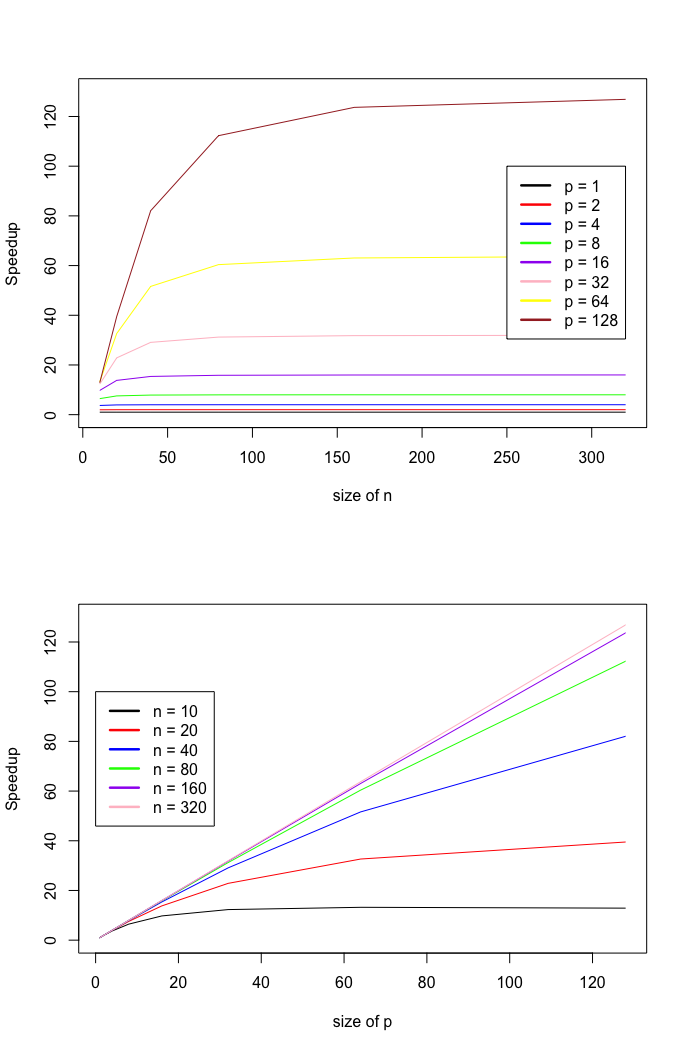
\includegraphics[width=1\textwidth]{speedup.png}
    \caption{This figure shows the speedup for constant p, respectively constant n.}
    \label{fig:speedup}
\end{figure}

\section{2.19 - Scalability}
\section{2.20 - Linear speedup and strong scalability}
\section{2.23 - Alternative algorithm for computing histogram}
\addcontentsline{toc}{section}{\refname}
\bibliography{references}

\end{document}
